\section{Experimental Evaluation}
\label{sec:exp}

{\bf Experimental environment.} All experiments in this section were
conducted on an 8-slave in-house Open Stack cloud, using Linux Ubuntu
14.04 and Spark v1.4.  Each node has 4 cores and 16 GB of RAM.  Spark
Standalone cluster manager and Hadoop 2.6 were used.

Because Spark is a lazy evaluation system, a \insql{materialize}
operation was appended to the end of each query, which consisted of
the count of nodes and edges.  In cases where the goal was to evaluate
a specific operation in isolation, we used warm start, which consisted
of materializing the graph upon load.  Each experiment was conducted 3
times, we report the average running time, which is representative
because we took great care to control variability.  Standard deviation
for each measure is at or below 5\% of the mean except in cases of
very small running times.

{\bf Data.}  We evaluate performance of our framework on two real
open-source datasets.
%\begin{enumerate}%[leftmargin=*]
%\item 
DBLP~\cite{dblp} contains co-authorship information from 1936 through
2015, with over 1.5 million author nodes and over 6 million undirected
co-authorship edges.  Total data size: 250 MB.
%
nGrams~\cite{nGrams} contains word co-occurrence information from 1520
through 2008, with over 1.5 million word nodes and over 65 million
undirected co-occurrence edges.  Total data size: 40 GB.  

\eat{
\item
  DELIS\footnote{\url{law.di.unimi.it/webdata/uk-union-2006-06-2007-05}}
  contains monthly snapshots of a portion of the Web graph focusing on
  the .uk domains from 05/2006 through 05/2007, with a total of over
  133 million nodes and over 5.5 billion directed edges\cite{BSVLTAG}.
  Data size: 1 TB.
}
%\end{enumerate}

The nGrams dataset is of comparable size to the LiveJournal dataset
in~\cite{Xin2013} and is commensurate with our cluster size.  DBLP and
nGrams differ not only in size, but also in the evolutionary
properties: co-authorship network nodes and edges have limited
lifespan, while the nGrams network grows over time, with nodes and
edges persisting for long duration.  All figures in the body of this
section are on the larger nGrams dataset.  Refer to the Appendix for
the DBLP figures, which show similar trends as nGrams.\eat{ We plan to
  carry out further experiments with a larger
  DELIS\footnote{\url{law.di.unimi.it/webdata/uk-union-2006-06-2007-05}}
  dataset as we grow the cluster in the near future.}

\subsection{Number of partitions}

\begin{figure*}[th!]
\centering
\begin{minipage}{3in}
  \centering
  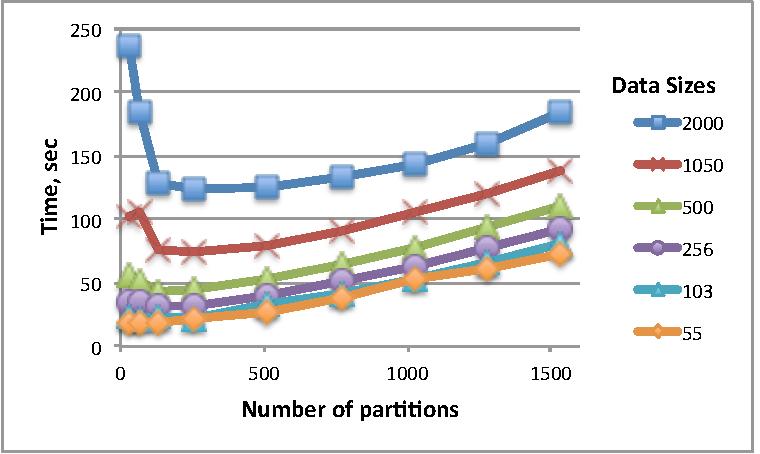
\includegraphics[width=2.7in]{figs/numparts.pdf}
\vspace{-0.1in}
  \caption{Load time vs. \# of partitions.}
  \label{fig:numparts}
\vspace{-0.1in}
\end{minipage}
\begin{minipage}{3in}
  \centering
  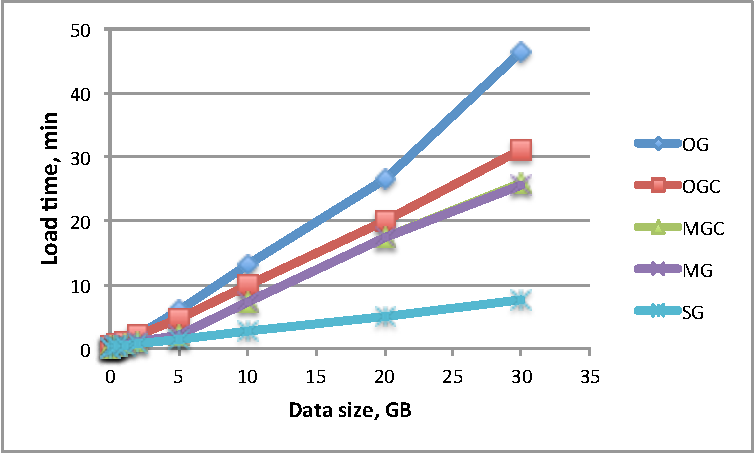
\includegraphics[width=2.7in]{figs/tselect.pdf}
\vspace{-0.1in}
  \caption{Load time vs. data size, nGrams.}
  \label{fig:tselect}
\vspace{-0.1in}
\end{minipage}
\end{figure*}

In Spark applications, one of the most influential performance drivers
is the choice of the number of partitions.  The default number of
partitions, based on the Hadoop block size, proved inefficient in
practice.  We extended GraphX for parallel reading of multiple files
with a custom number of partitions.  Further, we conducted a tuning
experiment, and developed a dynamic data size-based estimator of the
number of partitions.\eat{  We describe this experiment next, and use its
result to tune the number of partitions in all experiments in this
section.}

The tuning experiment consisted of running a simple \insql{TSelect}
query with each data structure, varying the number of partitions on
load for a range of data sizes.  In each data structure, we observe
the same trend -- as the number of partitions is increased for a given
data size, system performance quickly improves, but then starts to
deteriorate (Figure~\ref{fig:numparts}).  There is roughly a linear
relationship between data size and the best number of partitions (see
Figure~\ref{fig:partsfit} in the Appendix), which allowed us to fit a
linear function and use it to tune the number of partitions in all
experiments.

\subsection{Data loading}

To understand how different data structures perform as a function of
data size, we ran the following query on nGrams:

\begin{small}
\begin{verbatim}
      TSelect V[vid:int, word:str]; 
              E[vid1:int, vid2:int, cnt:int]
      From    data/nGrams
      Into    nGrams
      TWhere  Start >= x and End <= y
\end{verbatim}
\end{small}

\noindent where \insql{x} and \insql{y} parameters were varied to
achieve approximate desired data sizes for edge files.  Our file
format is a node file and an edge file per snapshot, with a node/edge
per line, respectively.  This format favors the SG data structure
because no data transformation, such as aggregation, is required.
This is substantiated experimentally, as can be seen in
Figure~\ref{fig:tselect}.  SG is the fastest data structure for data
loading, although all exhibit a linear increase as a function of data
size.\eat{ We observed the same trend in DBLP.}  Miao et
al.~\cite{DBLP:journals/tos/MiaoHLWYZPCC15} showed that data format
plays a significant role in load performance.  This is supported by
our results in Figure~\ref{fig:tselect}, and warrants development of
alternative file formats, which is in our immediate plans.

As we will see, load/materialize time makes up a significant portion
of the over-all time.  For this reason, all experiments that evaluate
performance of individual \ql operators are executed with a warm
start.

\eat{The significant influence of data format on data structure performance
has been shown previously~\cite{DBLP:journals/tos/MiaoHLWYZPCC15}.
Given the significant difference at size (3-5x) between SG and the
other data structures, an alternative file format for aggregated data
structures is warranted.}  

\eat{ Because the load/materialize time varies so significantly
  between different data structures, all subsequent experiments are
  reported with a warm start, with application of a desired
  partitioning strategy included during the loading process.}

\subsection{\insql{TSelect} with \insql{TGroup}}
\label{sec:exp:tgroup}

To investigate the comparative performance of different data
structures and partition strategies on the \insql{TGroup} operation, we used
the following query:

\begin{small}
\begin{verbatim}
      TSelect Any V[vid, any(word)];
              Any E[vid1, vid2, sum(cnt) as score]
      From    nGrams
      TWhere  Start >= x And End <= y
      TGroup  by 8 years
\end{verbatim}
\end{small}

We kept the aggregation time window fixed (8 years) and varied the
total number of snapshots in powers of 2.  Each snapshot contains
about 13 million edges.

Recollect that \insql{TGroup} requires a union and group by operation
in SG, a combination of transform with filter and group by for MG, and
transform with filter for OG.  Due to compactness, MGC outperforms MG
and OGC outperforms OG.  All data structures and partitioning
strategies show linear increase in structural aggregation time as the
number of snapshots grows.  As expected, because OGC is an already
aggregated data structure, it outperforms MGC and SG for the
\insql{TGroup} operation by up to two orders of magnitude.  This is
shown in Figure~\ref{fig:tgroupe}, where we present only the
best-performing variant (column-store) and partitioning strategy for
each data structure.

\begin{figure*}[t!]
\centering
\begin{minipage}{3in}
  \centering
  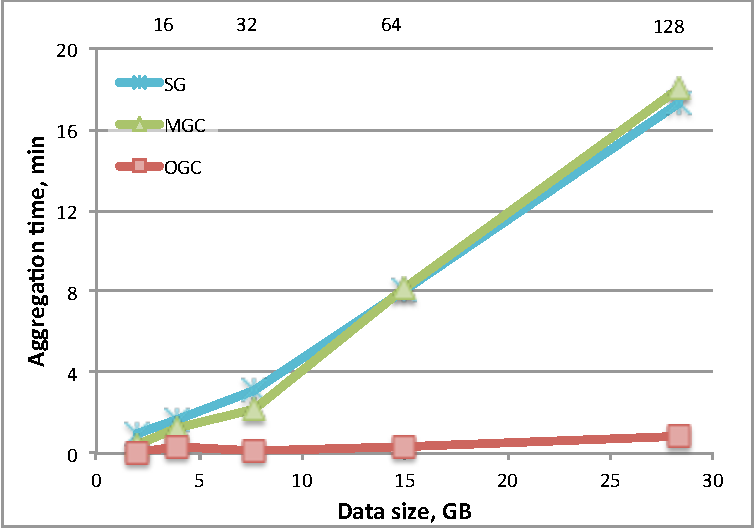
\includegraphics[width=2.5in]{figs/tgroupe_warm.pdf}
\vspace{-0.1in}
  \caption{\insql{TGroup} with \insql{Any} (warm start).}
  \label{fig:tgroupe}
\vspace{-0.1in}
\end{minipage}
\begin{minipage}{3in}
  \centering
  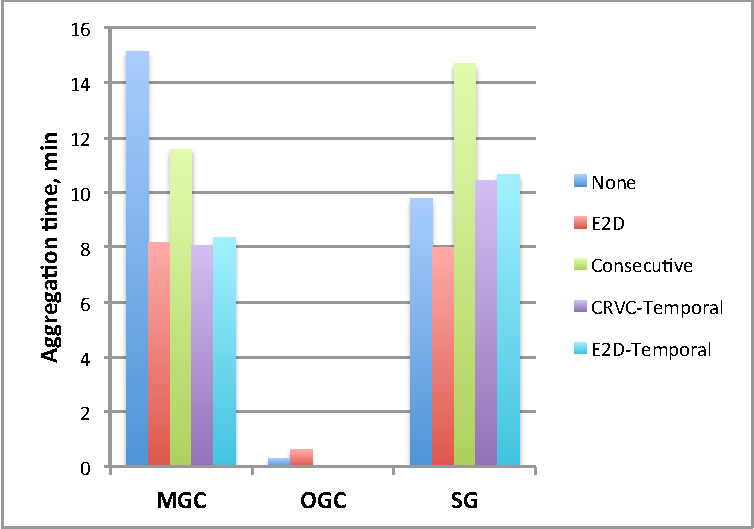
\includegraphics[width=2.5in]{figs/tgroupeparts.pdf}
\vspace{-0.1in}
  \caption{\insql{TGroup} by partitioning strategy.}
  \label{fig:tgroupeparts}
\vspace{-0.1in}
\end{minipage}
\end{figure*}

To compare between partitioning strategies, consider
Figure~\ref{fig:tgroupeparts}, which contains performance for each
data structure and strategy at 64 snapshot aggregation.  (The same
pattern is observed at all aggregation sizes.)  Partitioning
strategies improve performance for MGC on this operation --- all
outperform the default no partitioning case by 20\% or more.  This can
be explained by the group by operation that is performed on the edges.
E2D always places two edges with the same key in the same partition,
which leads to least cross-partition communication during aggregation.
Hybrid strategies use the aggregation window as the width of the run,
also placing the edges that are to be grouped in the same set of
partitions.  The differences between E2D and the hybrid strategies for
MGC are not significant.  E2D also does best for SG, but the gains are
smaller than for MGC.  We observed the same trend for the
\insql{TGroup} query with \insql{All} semantics --- see Appendix.

To demonstrate why we use warm start, consider
Figure~\ref{fig:tgroupe_cold} where the fastest partition condition
for each data structure is depicted (and is None in all 3 cases), and
note that loading time dominates the overall time, which also includes
partitioning, temporal aggregation, and materialization.  Based on
this figure alone, one would conclude that SG is the most efficient
data structure.  However, recall that the file format favors SG, and
so no conclusions about the performance of data structures for
individual operations should be drawn from cold start total time
alone.  \eat{Additionally, the fastest time for each data structure
  with cold start is achieved without applying a partition strategy
  because the process of partitioning takes additional non-trivial
  time. Thus, partition strategies for individual operations cannot be
  effectively compared from cold start data either.}

OGC outperforms the other data structures when we fix the data size
and vary the aggregation width.\eat{, as can be seen in
  Figure~\ref{fig:tgroupe_width}.}  OGC is insensitive to aggregation
width, with a slight improvement as the width increases.  SG and MGC
show a linear increase, with a drop for the final aggregation by the
whole size.  This trend is observed in both datasets, see Appendix for
figures.

\begin{figure*}
\centering
\begin{minipage}{3in}
  \centering
  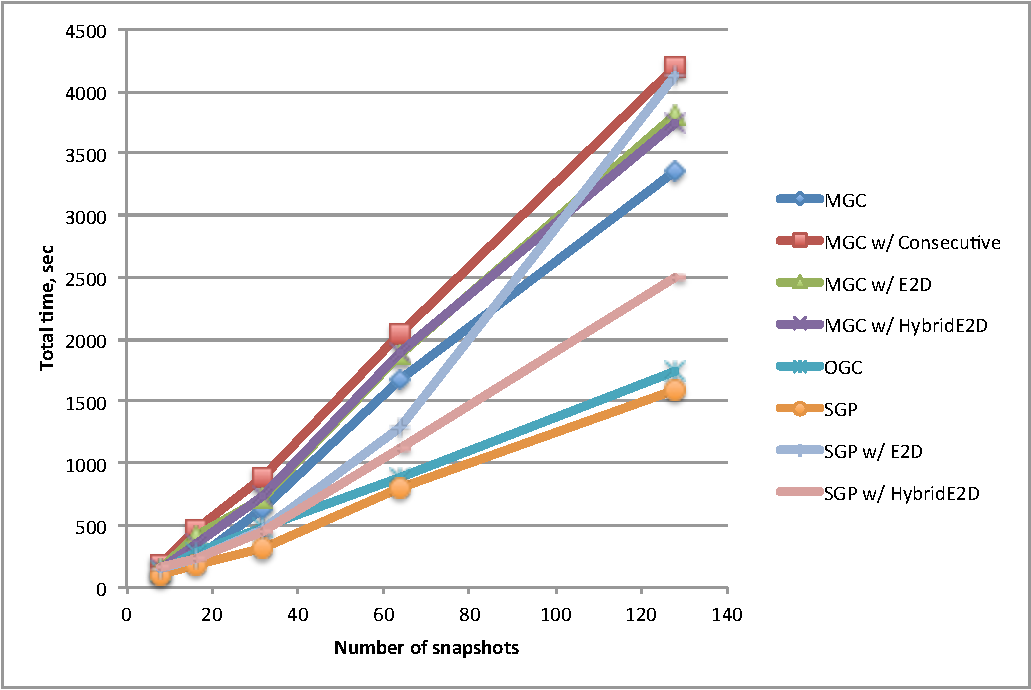
\includegraphics[width=2.5in]{figs/tgroupe_cold.pdf}
\vspace{-0.1in}
  \caption{\insql{TGroup} with \insql{Any} (cold start).}
\label{fig:tgroupe_cold}
\vspace{-0.1in}
\end{minipage}
\begin{minipage}{3in}
  \centering
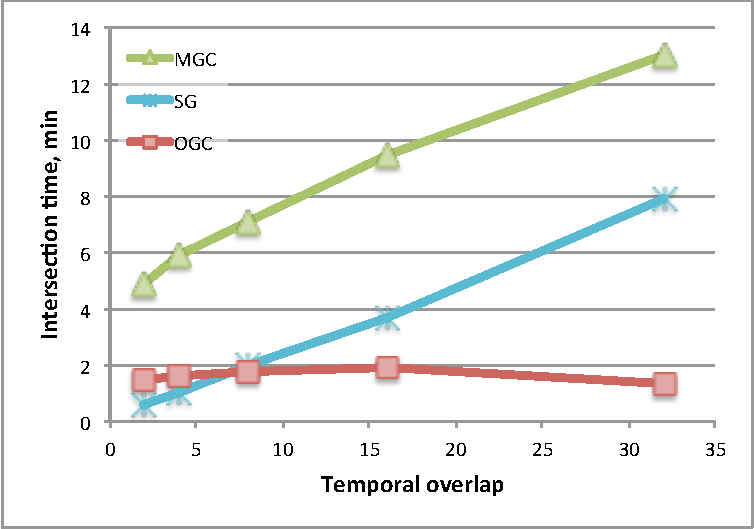
\includegraphics[width=2.5in]{figs/tand_all_warm.pdf}
\vspace{-0.1in}
\caption{\insql{TAnd} time vs. temporal overlap.}
\label{fig:tandall}
\vspace{-0.1in}
\end{minipage}
\end{figure*}

\subsection{\insql{TAnd} with \insql{All}}

\insql{TAnd} is a binary operation, and thus co-partitioning of the
\tgs should improve performance.  In this experiment we use the query:

\begin{small}
\begin{verbatim}
      TSelect All V[vid, max(word)];
              All E[vid1, vid2, max(cnt) as score]
      From    ( TSelect V; E
                From nGrams
                TWhere  Start >= x And End <= y )
              TAnd
              ( TSelect V; E
                From nGrams
                TWhere  Start >= n And End <= m )      
\end{verbatim}
\end{small}

We are selecting the two graphs from the same dataset and varying the
amount of temporal overlap (\insql{n - m}).  Note that this is the
worst-case scenario for structural aggregation with \insql{All}, since
the size of the intersection among the corresponding pairs of
snapshots is the highest possible.  Note that, while this query is a
good candidate for query rewriting, we did not optimize it in this
experiment, but executed it directly as specified.

\insql{TAnd} performs structural aggregation of for each snapshot pair
in SG, and one structural aggregation in all other data structures.
As the temporal overlap between the two graphs increases, we expect
OGC to outperform SG, and this is what we observe experimentally
(Figure~\ref{fig:tandall}).  SG outperforms other representations when
overlap is 7\% or lower, while OGC significantly outperforms SG and
MGC for higher overlap values.

Partitioning has a mild benefit for MGC, especially with the E2D
strategy, as it does for OGC and SG. See Figure~\ref{fig:tand_parts}
in the Appendix for side-by-side comparison.

\eat{
\begin{figure}[t!]
 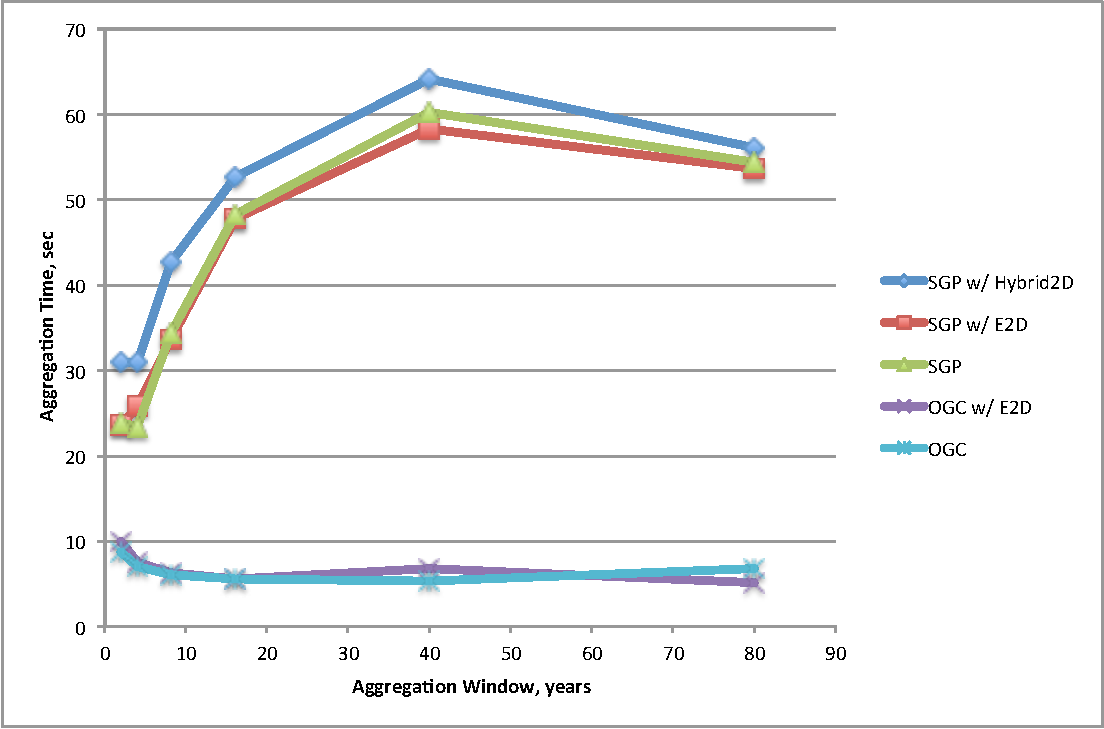
\includegraphics[width=2.7in]{figs/tgroupewidth.pdf}
 \caption{\insql{TGroup} time vs. aggregation width.}
 \label{fig:tgroupe_width}
\end{figure}
}

\insql{TOr} performance with \insql{Any} exactly matches that of
\insql{TAnd} with \insql{All} above, and we do not show it here.

\subsection{PageRank}

Snapshot analytics like PageRank are implemented using
the Pregel API in GraphX, with batch mode for MGC and OGC.  We used
the following query to evaluate data structure performance over
varying number of snapshots:

\begin{small}
\begin{verbatim}
      TSelect V[vid, pagerank()];
              E[vid1, vid2]
      From    nGrams
      TWhere  Start >= x And End <= y
\end{verbatim}
\end{small}

PageRank was executed for 10 iterations or until convergence,
whichever came first.  Performance of Pregel-based algorithms depends
heavily on the partition strategy, with best results achieved where
cross-partition communication is small.  For this reason, we evaluated
only no partitioning and E2D.

SG performs better than the other data structures in this experiment,
contrary to our expectation that batch mode of MGC and OGC would be
faster (Figure~\ref{fig:pagerank}).  This can be explained by MGC and
OGC using significantly more cross-partition communication due to the
following factors:

\begin{enumerate}[leftmargin=*]
\item Each individual snapshot is less dense than the aggregate
  (although this depends on the rate of change), and dense graphs do
  worse with Pregel analytics.
\item Individual snapshots are smaller and take fewer partitions, so
  less communication happens across partitions.
\item PageRank gets faster as vertex values converge, because those
  vertices stop sending out new messages.  In OGC/MGC a vertex converges
  only when it does so in all snapshots.
\eat{\item Messages for OGC are larger --- it is more costly to send a Map
  object than a number.}
\end{enumerate}

\begin{figure*}[t]
\centering
\begin{minipage}{3in}
  \centering
  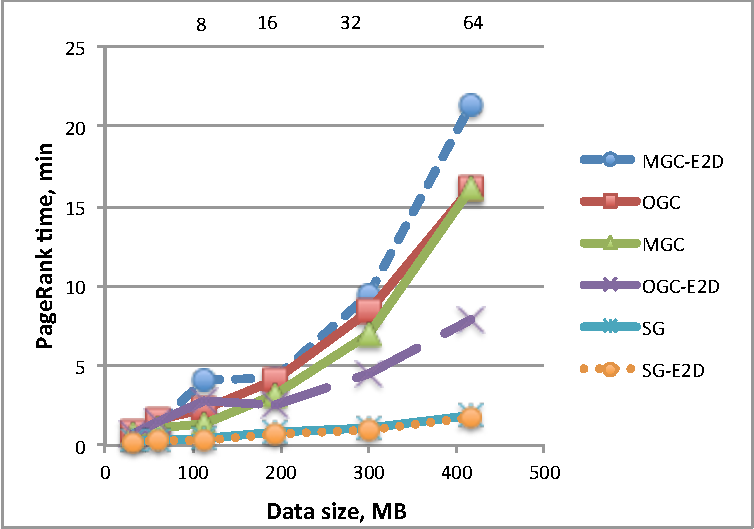
\includegraphics[width=2.6in]{figs/pagerank.pdf}
  \vspace{-0.1in}
  \caption{PageRank time.}
  \label{fig:pagerank}
  \vspace{-0.1in}
\end{minipage}
\begin{minipage}{3in}
  \centering
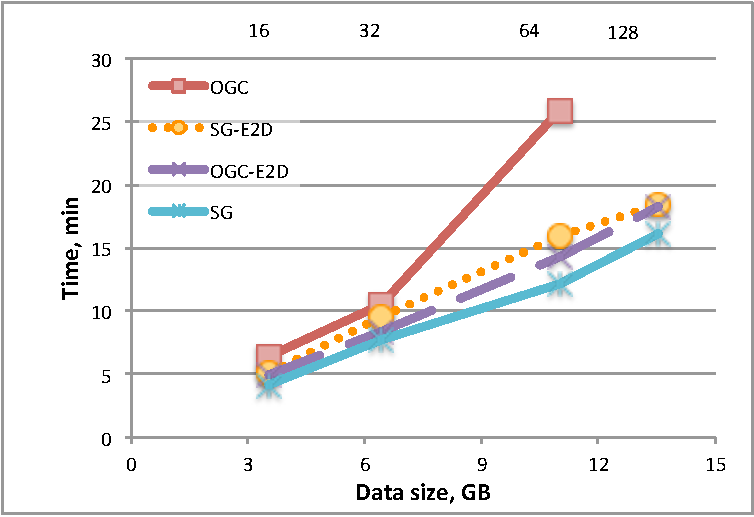
\includegraphics[width=2.6in]{figs/complexq.pdf}
  \vspace{-0.1in}
\caption{\insql{TGroup}, PageRank, trend.}
\label{fig:complexq}
  \vspace{-0.1in}
\end{minipage}
\end{figure*}

E2D partitioning leads to performance improvements in all data
structures except MGC.

\subsection{\insql{TSelect} with \insql{trend(pagerank())}}

All the experiments so far evaluated performance of individual \ql
operations. We conclude this section with a cold-start execution of
the query:

\begin{small}
\begin{verbatim}
      Select vid, pr
      From (TSelect Any V[vid, trend(prank) as pr]
                    Any E
            From (TSelect All V[vid, pagerank() as prank]; 
                          All E
                  From nGrams
                  TWhere Start >= x And End <= y
                  TGroup by 8 years)
            TGroup by size).toVerticesFlat()
      Order by pr
      Limit 10
\end{verbatim}
\end{small}

As we saw above, SG outperforms other representations for data load
and for PageRank, while OGC is very efficient for temporal
aggregation.  This query combines all of these operations, and adds a
trend analytic, and a transformation of the vertices of the result
into a flat vertex relation.

SG with no partitioning, and OGC with E2D show comparable
performances, as seen in Figure~\ref{fig:complexq}.

\eat{
\begin{figure}[t]
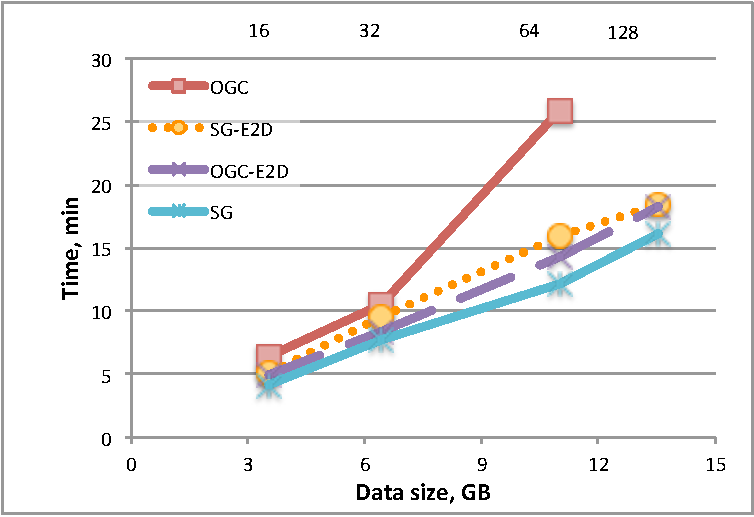
\includegraphics[width=3.2in]{figs/complexq.pdf}
\caption{Complex query: \insql{TGroup}, PageRank, trend.}
\label{fig:complexq}
\end{figure}
}

{\bf In summary,} no one data structure is most efficient across all
operations.  SG is most efficient for data load, because our file
format favors this data structure, and for PageRank.  OGC is most
efficient for temporal group and join.  The two data structures
perform comparably for the complex query.  E2D is the most efficient
partitioning method in most cases, and E2D-Temporal is a close second.
